\section{映射的局部结构}
\label{sec:mrel-local-structure}

要判断一个映射的像或原像能否成为光滑子流形，先要看映射在一点附近怎样作用于方向。微分可能把非零的切向量送到零，丢失方向；可能达不到目标的全部方向；还可能在附近各点的秩不同。本节的$M,N$都是无边界光滑流形，维数分别为$m,n$，整体的拓扑条件留到下一节。

\subsection{浸入与淹没}
\label{sec:mrel-immersion-submersion}

\paragraph{定义}
线性代数里，矩阵的列线性无关时对应的映射是单射，行线性无关时是满射。下面两个矩阵分别属于这两类：
\[
\begin{bmatrix}1&0\\0&1\\1&1\end{bmatrix},\qquad
\begin{bmatrix}1&0&1\\0&1&1\end{bmatrix}.
\]
第一个是$3\times2$矩阵，秩为$2$，把$\mathbb R^2$单射地送进$\mathbb R^3$；第二个是$2\times3$矩阵，秩为$2$，把$\mathbb R^3$满射地压到$\mathbb R^2$上。对映射在每一点的微分提出这两种要求，就得到两类映射。

\begin{definition}[浸入与淹没]
\label{def:mrel-immersion-submersion}
设$F:M\to N$光滑。若对每个$p\in M$，$\mathrm dF_p$都是单射，则称$F$为\term{浸入}（immersion）；若对每个$p\in M$，$\mathrm dF_p$都是满射，则称$F$为\term{淹没}（submersion）。
\end{definition}

浸入不丢失方向：经过$p$的两个不同速度被送到$F(p)$处的两个不同速度。淹没覆盖方向：$F(p)$处的任何速度都是某个$p$处速度的像。用秩表达，浸入在每点秩为$m$，淹没在每点秩为$n$。

单射要求$m\leq n$，满射要求$m\geq n$，所以浸入只能从低维到高维或同维，淹没只能从高维到低维或同维。同维时两者一致，由反函数定理都等价于局部微分同胚。

\paragraph{例子}
曲线$\gamma:I\to M$是浸入，当且仅当速度处处非零。图~\ref{fig:mrel-cusp-velocity}比较了两条平面曲线。$E(t)=(\cos t,\sin t)$作为$\mathbb R\to\mathbb R^2$的映射，速度$(-\sin t,\cos t)$的长度恒为$1$，处处非零，是浸入。

$\beta(t)=(t^2,t^3)$的速度是$(2t,3t^2)$，在$t=0$处为零，不是浸入。它的像是曲线$y_2^2=y_1^3$，在原点有一个尖点。接近原点时速度越来越小，曲线的方向在原点处从一支突然转到另一支，这正是速度为零允许发生的事。

\begin{BookInlineFigure}
  \centering
  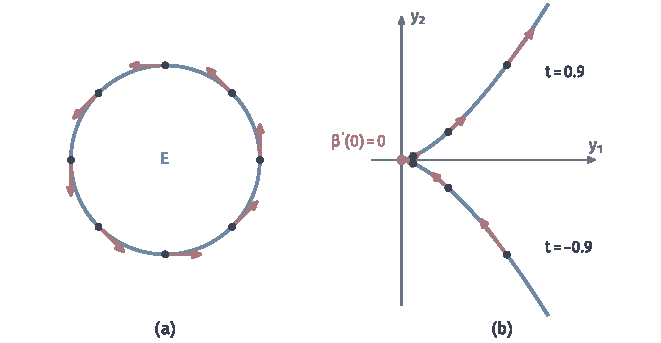
\includegraphics[width=112mm]{figures/04-spaces-measures-and-geometry/04-manifolds/matplotlib/mrel-cusp-velocity/figure.pdf}
  \caption{速度是否为零。(a)$E(t)=(\cos t,\sin t)$的速度（红箭头）长度恒为$1$，$E$是浸入。(b)$\beta(t)=(t^2,t^3)$在$t=\pm0.3,\pm0.6,\pm0.9$处的速度按真实长度的$0.12$倍画出，越接近原点越短；原点处速度为零，曲线出现尖点。}
  \label{fig:mrel-cusp-velocity}
\end{BookInlineFigure}

高维的浸入也可以手算。北极球极投影的逆把坐标$\bm u=(u_1,u_2)$送到$\mathbb R^3$，记$\rho=u_1^2+u_2^2$，
\[
\sigma_N^{-1}(\bm u)=\frac{(2u_1,\ 2u_2,\ \rho-1)}{\rho+1}.
\]
在$\bm u=(0,3)$处，第一列已在第~\ref{chap:manifold-basics}章算出是$(\tfrac15,0,0)$。第二列对$u_2$求导，三个分量分别是
\[
\frac{-4u_1u_2}{(\rho+1)^2}=0,\qquad
\frac{2(\rho+1)-4u_2^2}{(\rho+1)^2}=-\frac4{25},\qquad
\frac{4u_2}{(\rho+1)^2}=\frac3{25}.
\]

于是在这一点的Jacobian矩阵及其秩是
\[
\bm J=\begin{bmatrix}1/5&0\\0&-4/25\\0&3/25\end{bmatrix},\qquad \operatorname{rank}\bm J=2.
\]
两列正是切向量$\bm v$与$\bm w$，这个$3\times2$矩阵列满秩，所以$\sigma_N^{-1}$在这一点是单射的微分。

淹没的例子是投影。取前$n$个坐标的映射$\pi:\mathbb R^m\to\mathbb R^n$，$m\geq n$，Jacobian矩阵是$[\bm I_n\ \bm 0]$，行满秩。球面上的高度函数$h$是更有几何意味的例子，它在北极图中的表示和微分系数是
\[
h\circ\sigma_N^{-1}(\bm u)=\frac{\rho-1}{\rho+1},\qquad
\mathrm dh=\frac{4u_1\,\mathrm du_1+4u_2\,\mathrm du_2}{(\rho+1)^2}.
\]

在$\bm u=(0,3)$处系数是$(0,0.12)$，非零，秩为$1$。在$\bm u=\bm 0$（南极）处系数全为零，秩为$0$；北极由南极图同样算出秩为$0$。所以$h:S^2\to\mathbb R$不是淹没，但限制到$S^2\setminus\{N,S\}$上就是淹没。

图~\ref{fig:mrel-height-rank}读出同一件事的几何含义。在$p$处，沿纬线的方向$\bm e_1=(1,0,0)$不改变高度，构成微分的核；沿经线向下的单位方向$\bm e_2=(0,0.8,-0.6)$让高度以$-0.6$的速率变化，覆盖了$\mathbb R$的全部方向。淹没的等值集正是纬线这样的一维曲线，维数$2-1=1$。

\begin{BookInlineFigure}
  \centering
  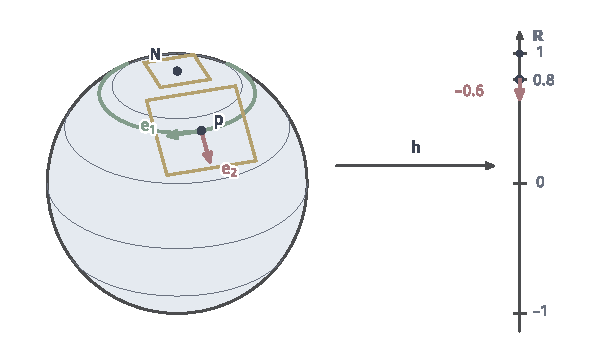
\includegraphics[width=104mm]{figures/04-spaces-measures-and-geometry/04-manifolds/matplotlib/mrel-height-rank/figure.pdf}
  \caption{高度函数$h(\bm y)=y_3$在$S^2$上的秩。在$p=(0,\tfrac35,\tfrac45)$处，绿色的纬线方向$\bm e_1$属于$\ker\mathrm dh_p$，红色的方向$\bm e_2$被送到$\mathbb R$上长度$0.6$的向量（两侧都按真实长度的$0.3$倍画出）。在北极$N$处切平面水平，$\mathrm dh_N=0$，所有方向都被送到零。}
  \label{fig:mrel-height-rank}
\end{BookInlineFigure}

\paragraph{微分的单射、满射与映射的单射、满射}
浸入与淹没都是逐点关于微分的条件，不涉及映射本身是否单射或满射。表~\ref{tab:mrel-injective-comparison}列出了四个例子，说明这两组概念互相独立，判断时要分清问的是方向还是点。

\begin{BookInlineTable}
  \centering
  \begin{tabular}{lll}
    \toprule
    映射 & 映射本身 & 微分\\
    \midrule
    $E:\mathbb R\to\mathbb R^2$ & 非单射（周期$2\pi$） & 处处单射\\
    $\beta(t)=(t^2,t^3)$ & 单射 & 在$t=0$处不单射\\
    $h:S^2\setminus\{N,S\}\to\mathbb R$ & 非满射（像为$(-1,1)$） & 处处满射\\
    $x\mapsto x^3$ & 满射 & 在原点不满射\\
    \bottomrule
  \end{tabular}
  \caption{映射的单射、满射与微分的单射、满射互相独立。}
  \label{tab:mrel-injective-comparison}
\end{BookInlineTable}

\subsection{常秩定理}
\label{sec:mrel-constant-rank}

\paragraph{一点的秩与邻域中的秩}
线性代数告诉我们，任何秩为$r$的矩阵$\bm A$，在定义域和值域各选一组合适的基之后，都成为最简单的形式：存在可逆矩阵$\bm P,\bm Q$，使
\[
\bm P\bm A\bm Q=\begin{bmatrix}\bm I_r&\bm 0\\\bm 0&\bm 0\end{bmatrix}.
\]
选基换成选坐标，我们希望非线性映射也能写成$(x_1,\ldots,x_r,0,\ldots,0)$这样的形式。

类比在这里遇到了线性代数没有的问题：Jacobian矩阵随点变化，矩阵的秩也可能随点变化。一点的秩控制附近秩的下限，却不控制上限。若$\mathrm dF_p$的秩为$r$，Jacobian矩阵有一个非零的$r$阶子式，子式是偏导数的多项式，连续，所以在$p$附近仍非零，附近各点的秩至少为$r$。

秩却可以在$p$附近变大。$f(x)=x^2$在$0$处秩为$0$，在其余点秩为$1$。若它在$0$附近有秩$1$的标准形式$x\mapsto x$，就应当局部单射；若有秩$0$的标准形式，就应当局部为常值。这两者都不成立，因为$f(1/k)=f(-1/k)$，而$f$又不是常值。可见只看一点的秩，得不到局部形式。

二维的例子也一样。令$F(x,y)=(x,xy)$，Jacobian矩阵和行列式分别是
\[
\bm J_F=\begin{bmatrix}1&0\\y&x\end{bmatrix},\qquad \det\bm J_F=x.
\]
在$x=0$处秩为$1$，在$x\neq0$处秩为$2$。球面的高度函数也是如此：在两极秩为$0$，在附近的点秩为$1$，所以两极附近不能用单一的标准形式描述。

有一个重要的例外是满秩。秩不能超过$\min(m,n)$，若$p$处的秩已经达到$\min(m,n)$，附近的秩既不小于它，也不能更大，只能保持不变。所以对浸入和淹没，一点满秩就推出邻域常秩，下面的定理对它们自动适用。

\paragraph{定理与证明}
常秩条件下，映射在适当的坐标中就是线性映射的标准形式。证明的想法是用反函数定理逐步“拉直”：先在源中换坐标，使映射的前$r$个分量变成坐标本身；再由秩的上限，说明其余分量只依赖前$r$个坐标；最后在目标中换坐标，把其余分量减掉。

\begin{theorem}[常秩定理]
\label{thm:mrel-constant-rank}
设$F:M\to N$光滑，$p\in M$，$F$在$p$的某个邻域中各点的秩都等于$r$。则存在以$p$为中心的图$(U,\varphi)$与以$F(p)$为中心的图$(V,\psi)$，$F(U)\subseteq V$，使
\begin{equation}
\psi\circ F\circ\varphi^{-1}(x_1,\ldots,x_r,x_{r+1},\ldots,x_m)=(x_1,\ldots,x_r,0,\ldots,0).
\label{eq:mrel-constant-rank-form}
\end{equation}
\end{theorem}

\begin{proof}
取两侧的图，可设$F$是欧氏开集$W\subseteq\mathbb R^m$到$\mathbb R^n$的光滑映射，$p=\bm 0$，$F(\bm 0)=\bm 0$，并且在$W$上秩恒为$r$。$\bm J_F(\bm 0)$有一个非零的$r$阶子式，重排两侧坐标的次序，可设它位于左上角。

把变量写成$\bm x=(\bm x',\bm x'')$，$\bm x'\in\mathbb R^r$，并把$F$写成$(Q,R)$，其中$Q$取值于$\mathbb R^r$。于是$\partial Q/\partial\bm x'(\bm 0)$可逆。

第一步，在源中换坐标。令$G(\bm x)=(Q(\bm x),\bm x'')$，它在$\bm 0$处的Jacobian矩阵是
\[
\bm J_G(\bm 0)=\begin{bmatrix}\partial Q/\partial\bm x'(\bm 0)&\partial Q/\partial\bm x''(\bm 0)\\\bm 0&\bm I_{m-r}\end{bmatrix},
\]
行列式等于$\det\partial Q/\partial\bm x'(\bm 0)\neq0$。由反函数定理，$G$把$\bm 0$的某个邻域微分同胚地映到$\bm 0$的一个邻域，缩小后可设后者是开方体$C$。

在$C$上有$G\circ G^{-1}=\mathrm{id}$，比较前$r$个分量得$Q(G^{-1}(\bm z))=\bm z'$，所以
\[
F\circ G^{-1}(\bm z)=\bigl(\bm z',\,\widetilde R(\bm z)\bigr),\qquad \widetilde R=R\circ G^{-1}.
\]

第二步，利用秩的上限。$F\circ G^{-1}$的Jacobian矩阵是
\[
\begin{bmatrix}\bm I_r&\bm 0\\\partial\widetilde R/\partial\bm z'&\partial\widetilde R/\partial\bm z''\end{bmatrix}.
\]
$G^{-1}$是微分同胚，所以这个矩阵的秩恒等于$r$。前$r$行已经贡献了秩$r$，若右下块有非零元素，秩就至少为$r+1$，于是
\[
\frac{\partial\widetilde R}{\partial\bm z''}\equiv\bm 0.
\]
$C$是方体，固定$\bm z'$时$\bm z''$在一个凸集中变化，所以$\widetilde R(\bm z)=S(\bm z')$只依赖$\bm z'$。

第三步，在目标中换坐标。令
\[
T(\bm y',\bm y'')=\bigl(\bm y',\ \bm y''-S(\bm y')\bigr),
\]
定义在$\bm y'$属于$C$在前$r$个坐标上的投影的开集上。它光滑，逆为$(\bm y',\bm y''+S(\bm y'))$，也光滑。代入后得到
\[
T\circ F\circ G^{-1}(\bm z)=\bigl(\bm z',\ S(\bm z')-S(\bm z')\bigr)=(\bm z',\bm 0).
\]
取源中的新坐标为$G$，目标中的新坐标为$T$，并缩小邻域使$F(U)\subseteq V$，即得所需形式。
\end{proof}

\paragraph{例子：一步步拉直}
证明中的三步可以在一个具体映射上完整走一遍。令$F:\mathbb R^2\to\mathbb R^2$，
\[
F(x_1,x_2)=(s,s^2),\qquad s=x_1+x_2.
\]
它的Jacobian矩阵第二行是第一行的$2s$倍：
\[
\bm J_F=\begin{bmatrix}1&1\\2s&2s\end{bmatrix},\qquad\operatorname{rank}\bm J_F=1.
\]
所以秩处处等于$1$，常秩定理适用，$r=1$。

这里$Q(x_1,x_2)=x_1+x_2$，$R(x_1,x_2)=(x_1+x_2)^2$，$\partial Q/\partial x_1=1\neq0$。第一步在源中换坐标，
\[
G(x_1,x_2)=(x_1+x_2,\ x_2),\qquad G^{-1}(z_1,z_2)=(z_1-z_2,\ z_2).
\]

把$G^{-1}$代入$F$，第一个分量变成坐标$z_1$，第二个分量自动只依赖$z_1$：
\[
F\circ G^{-1}(z_1,z_2)=(z_1,\ z_1^2).
\]
也就是说第二步中的$S(z_1)=z_1^2$，这里无需额外计算，因为$F$本来就沿直线$x_1+x_2=$常数取常值。第三步在目标中减去$S$，
\[
T(y_1,y_2)=(y_1,\ y_2-y_1^2),\qquad T\circ F\circ G^{-1}(z_1,z_2)=(z_1,0).
\]

图~\ref{fig:mrel-rank-steps}跟踪了点$(1,2)$：$F$把它送到$(3,9)$，$G$把它送到$(3,2)$，$T$把$(3,9)$送到$(3,0)$，而$(z_1,z_2)=(3,2)$在标准形式下正好变成$(3,0)$。图中可以看到映射的结构：源上的等值线是一族平行直线，目标上的像是一条抛物线，换坐标只是把直线摆正、把抛物线压平。

\begin{BookInlineFigure}
  \centering
  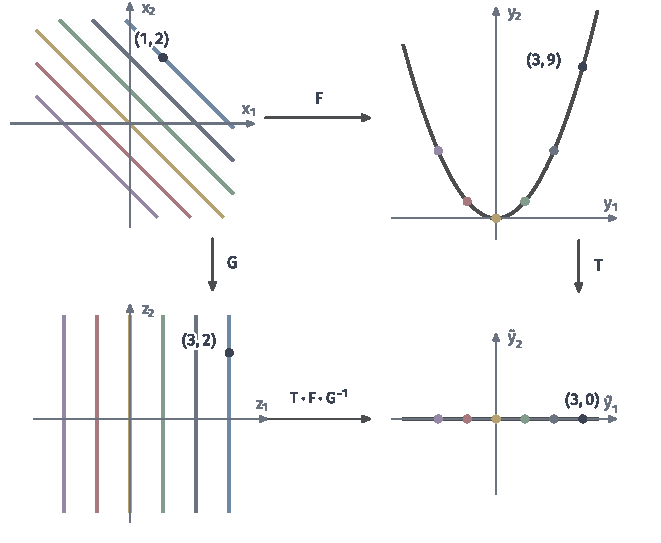
\includegraphics[width=112mm]{figures/04-spaces-measures-and-geometry/04-manifolds/matplotlib/mrel-rank-steps/figure.pdf}
  \caption{常秩定理的三步，$F(x_1,x_2)=(s,s^2)$，$s=x_1+x_2$。左上：源中的等值线$x_1+x_2=c$，$c=-2,\ldots,3$，同一条线上颜色相同。右上：它们被$F$压成抛物线上的一点（同色）。左下：$G$把等值线摆成竖直线。右下：$T$把抛物线压平到坐标轴上。黑点是$(1,2)$的轨迹。}
  \label{fig:mrel-rank-steps}
\end{BookInlineFigure}

\paragraph{浸入与淹没的局部形式}
由上面的满秩讨论，浸入在每点附近秩恒为$m$，淹没恒为$n$，常秩定理直接给出它们的局部形式：
\begin{align}
\text{浸入：}\quad&(x_1,\ldots,x_m)\mapsto(x_1,\ldots,x_m,0,\ldots,0),\label{eq:mrel-immersion-form}\\
\text{淹没：}\quad&(x_1,\ldots,x_n,\ldots,x_m)\mapsto(x_1,\ldots,x_n).\label{eq:mrel-submersion-form}
\end{align}

图~\ref{fig:mrel-normal-forms}画出这两种形式和一般常秩映射。式~\eqref{eq:mrel-immersion-form}说，浸入局部上把$\mathbb R^m$放进$\mathbb R^n$作为前$m$个坐标的子空间，所以局部单射，像的一小块是一片平的$m$维片。式~\eqref{eq:mrel-submersion-form}说，淹没局部上沿后$m-n$个坐标投影，每点的原像局部是一片$m-n$维的片。

\begin{BookInlineFigure}
  \centering
  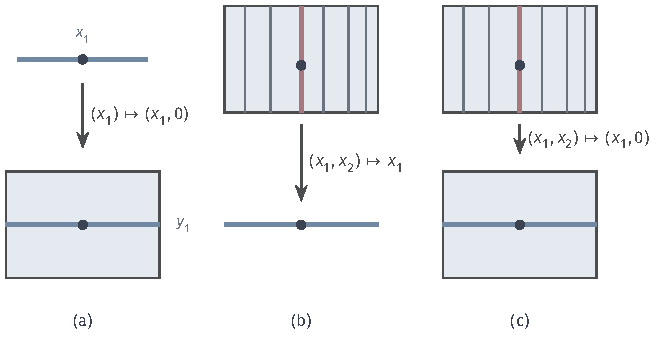
\includegraphics[width=111.767mm]{figures/04-spaces-measures-and-geometry/04-manifolds/tikz/mrel-normal-forms/figure.pdf}
  \caption{常秩映射的局部标准形式。(a)浸入：区间平放进平面，成为一条坐标线。(b)淹没：矩形沿竖直方向投影到区间上，红色竖线是一点的原像。(c)一般的常秩映射（$m=n=2$，$r=1$）：竖线整条压成一点，像是一条横线，定义域和值域都没有被占满。}
  \label{fig:mrel-normal-forms}
\end{BookInlineFigure}

前面的例子都可以写成这样的形式。对$E$，在圆周上用$\mathbb R^2$的极坐标图$(\theta,r-1)$，$E$的坐标表示恰好是$t\mapsto(t,0)$，这就是式~\eqref{eq:mrel-immersion-form}。对高度函数$h$，在$p$附近用坐标$(h,\lambda)$，其中$\lambda$是经度，$h$的坐标表示就是投影$(h,\lambda)\mapsto h$，这就是式~\eqref{eq:mrel-submersion-form}。

表~\ref{tab:mrel-immersion-submersion}把两种映射并排比较。下一节正是用这两种局部形式构造子流形：浸入给出“像”的局部坐标，淹没给出“水平集”的局部坐标。

\begin{BookInlineTable}
  \centering
  \begin{tabular}{lll}
    \toprule
    & 浸入 & 淹没\\
    \midrule
    微分 & 处处单射 & 处处满射\\
    秩 & 恒为$m$ & 恒为$n$\\
    维数 & $m\leq n$ & $m\geq n$\\
    Jacobian矩阵 & 列满秩 & 行满秩\\
    局部形式 & 加上若干零坐标 & 丢掉若干坐标\\
    局部几何 & 像是平的$m$维片 & 原像是平的$(m-n)$维片\\
    \bottomrule
  \end{tabular}
  \caption{浸入与淹没的比较。}
  \label{tab:mrel-immersion-submersion}
\end{BookInlineTable}
